%% (c) 2012 florian jung
%% (c) 2012 Robert Jonsson
%% we should consider putting this under a proper license. GPL, or
%% some GPL-like documentation license??

%% rules for editing documentation: (READ THIS FIRST)
%% ~~~~~~~~~~~~~~~~~~~~~~~~~~~~~~~~~~~~~~~~~~~~~~~~~~
%%
%% please try to let newly written lines be shorter than 72 characters.
%% minor exceptions are okay, but please not more than 80 chars.
%% comments shall start after character #80 of the line (that is,
%% they shall be "on the right margin")
%%
%% DON'T MIX up changes and reformatting in one commit. when changing
%% stuff, please don't touch the lines before and after your change
%% (that is, do not re-wrap them), even if it will look a bit patchy.
%% this is for being able to easily use diff.
%% when you want to reformat this file, then do it. but don't change
%% anything, as this would be hard to find in a diff. and clearly
%% state in the commit log that you "only" rearranged things.
%%
%% please adhere to the "User's manual" / "Internals" / "Design"
%% partitioning (genereally, don't change the chapters until there
%% is a really good reason for doing so (adding a chapter like
%% "feature requests" as flo did in r1497 IS one).
%% Below that, feel free to change the logical arrangement
%% (making paragraphs to subsections and similar) if you deem it
%% necessary.
%%
%% Whenever referring to code symbols, constants or source/header
%% files, please use \sym{someClass::someSymbol}, \usym{UPPERCASE_THING}
%% or \f{file.cpp}.
%% Only specify file paths or namespaces where it would be ambiguous
%% otherwise. Specify 'someClass::' until it would disturb the reader
%% and it is obvious. you have to replace '_' by {\_} (with the {}!).
%% These macros do automatic hyphenation on Camel-Case, under_-score
%% and scope::-operator boundaries. If you need to insert additional
%% hyphenation points, use {\-}.
%% Example: \sym{someClass::someAb{\-}nor{\-}mal{\-}lyLongName} will
%%          hyphenate: some-Class::-some-Ab-nor-mal-ly-Long-Name
%%
%% Whenever referring to URLs, please wrap them in \url{blah}. Key
%% combinations shall look like \key{CTRL+C}. Menu items shall look
%% like \menu{Menu > Submenu > Menu Item}.
%%
%% Where possible, reference other parts of this documents with
%% \label and \ref. Avoid duplicate information under "Internals" by
%% referring to the appropriate section in "User's manual".
%%
%% Please do no time-stamping of sections. if you need time-stamps,
%% use "svn blame documentation.tex"
%%
%% If you contribute something, feel free to add yourself to \author.
%%
%% If you don't speak LaTeX fluently, a few tips:
%% * \section, \subsection, \subsubsection, \paragraph, \subparagraph
%%   let you create sections etc. just copy-and-paste if unsure.
%% * you must prefix special characters like the underscore with \
%%   (backslash)
%% * \emph{some text} emphasizes the text, printing it italic.
%% * \texttt{some text} displays the text in a typewriter font
%% * \label{someName} creates a label at this position. this doesn't
%%   show up in the pdf. with \ref{someName}, you can reference to this
%%   label. (LaTeX will insert the section number instead of \ref)
%%   For this to work, you might need to recompile the .tex twice.
%%
%% 
%%%%%%%%%%%%%%%%%%%%%%%%%%%%%%%%%%%%%%%%%%%%%%%%%%%%%%%%%%%%%%%%%%%%%%%%
%%
%% Dependencies:
%% To produce pdf output from this document the following packages are
%% needed (atleast under Ubuntu derivatives)
%% latex???-base
%% texlive-latex-recommended
%% texlive-latex-extra
%%
%% To produce a pdf version of this manual type:
%% pdflatex documentation.tex <enter>
%% A file documentation.pdf should be generated.
%%
%%%%%%%%%%%%%%%%%%%%%%%%%%%%%%%%%%%%%%%%%%%%%%%%%%%%%%%%%%%%%%%%%%%%%%%%



\documentclass[a4paper]{report}
\usepackage[a4paper,  left=2.5cm, right=2.5cm, top=2.5cm, bottom=2.5cm]{geometry}
\usepackage[T1]{fontenc}
\usepackage[utf8]{inputenc}
\usepackage{lmodern}
\usepackage[english]{babel}
\usepackage{graphicx}
\usepackage{hyphenat}
\usepackage{wrapfig}
\usepackage{fancyhdr}
\usepackage{hyperref}
\usepackage{xcolor}
\hypersetup{
  linkcolor=blue,
  urlcolor=blue,
  colorlinks=true,         % hyperlinks will be blue
  linkbordercolor=blue,     % hyperlink borders will be blue
  %pdfborderstyle={/S/U/W 1} % border style will be underline of width 1pt
}
\pagestyle{fancy}
        \lhead{\scriptsize{\slshape\leftmark}}
        \chead{}
        \rhead{\thepage}
        \lfoot{}
        \cfoot{}
        \rfoot{}
        \renewcommand{\headrulewidth}{0.4pt}
\usepackage{ifthen}

% Hyphenate symbols before each uppercase letter, after each underscore
% (without a "-") and after each ':' (without a "-")
% TODO for any latex crack: also do automatic hyphenation, that is,
% instead of some-Automation-Expression, do some-Au-to-ma-tion-Ex-press-ion
\makeatletter
\newcommand{\camelhyph}[1]{\@fterfirst\c@amelhyph#1\relax }
\newcommand{\underscorehyph}[1]{\@fterfirst\u@nderscorehyph#1\relax }
\def\@fterfirst #1#2{#2#1}
\def\c@amelhyph #1{%
\ifthenelse{\equal{#1}\relax}{}{%  Do nothing if the end has been reached
  \ifnum`#1=95 \_\hspace{0pt}\else      %     Check whether #1 is "_", then print _[thin space]
    \ifnum`#1=58 :\hspace{0pt}\else
      \ifnum`#1>64
        \ifnum`#1<91 \-#1\else#1\fi%     Check whether #1 is an uppercase letter,
      \else#1\fi
    \fi
  \fi
                            %     if so, print \-#1, otherwise #1
  \expandafter\c@amelhyph%    %     insert \c@amelhyph again.
}}
\def\u@nderscorehyph #1{%
\ifthenelse{\equal{#1}\relax}{}{%  Do nothing if the end has been reached
  \ifnum`#1=95 \_\hspace{0pt}\else      %     Check whether #1 is "_", then print _\-
    \ifnum`#1=58 :\hspace{0pt}\else#1\fi\fi
  \expandafter\u@nderscorehyph%    %     insert \u@nderscorehyph again.
}}
\makeatother



\author{Florian Jung, Robert Jonsson, Tim Donnelly}
\title{MusE Documentation}

% Orcan: not needed since the hyperref package takes care of all
%\newcommand{\url}[1]{\texttt{#1}}
\newcommand{\key}[1]{\textbf{#1}}
\newcommand{\shell}[1]{\texttt{\textbf{#1}}}
\newcommand{\menu}[1]{\textbf{#1}}
\newcommand{\sym}[1]{\texttt{\camelhyph{#1}}}
\newcommand{\listing}[1]{\texttt{\camelhyph{#1}}}
\newcommand{\usym}[1]{\texttt{\underscorehyph{#1}}}
\newcommand{\file}[1]{\texttt{\camelhyph{#1}}}
\newcommand{\screenshotwidth}[0]{0.8\textwidth}


\begin{document}
\begin{figure}[htp]
\centering 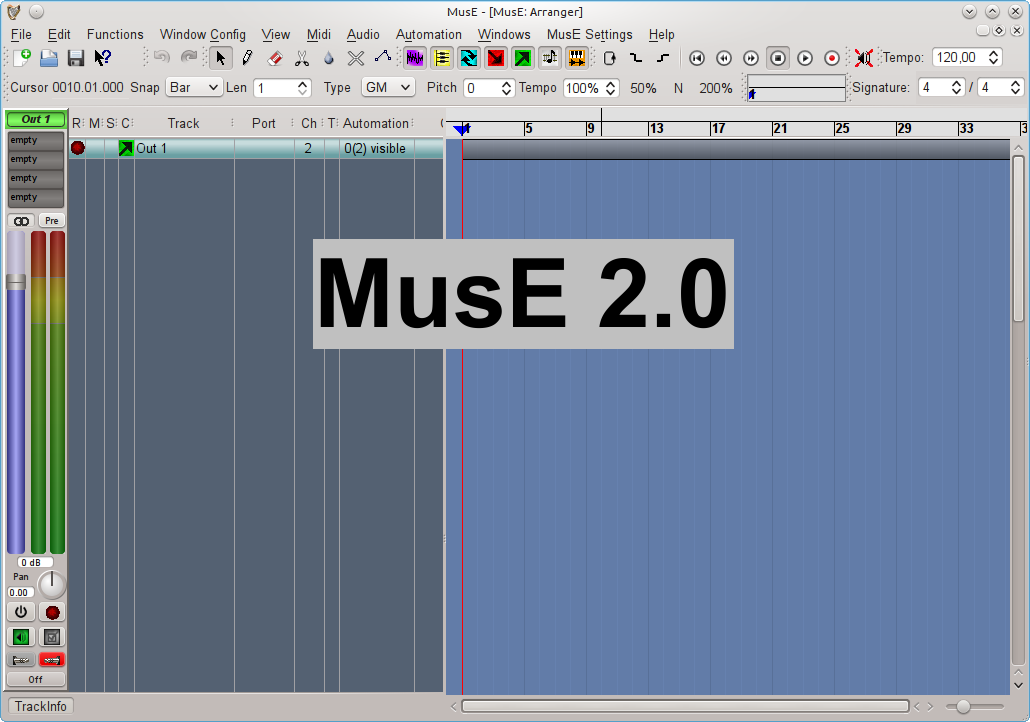
\includegraphics[width=1.0\textwidth]{pics/muse2}
\label{fig:MusE}
\end{figure}
\tableofcontents
\chapter{What is this?}
You are, if you have printed this document, holding in your hand the
written documentation for the audio and midi sequencer MusE version 2.\\ 
\url{http://www.muse-sequencer.org} is MusE's home on the internet where
everything MusE related should be possible to find, software, this
documentation, forums, mailing lists, bug reporting, FAQs. If you have
this document but not the software head on over there to find what it's
all about.
\chapter{User's manual}

\section{Introduction}
\subsection{A brief history of computer audio and MusE}
To quickly summarize over a decades open source development: in 1999 Werner
 Schweer released the first version of MusE, muse-0.0.1.tar.gz, in it's first
few releases (actually not few, Werner relentlessly churned out new releases)
MusE was only a midi sequencer. The target was to create a fully fledged
midi sequencer for the Linux operating system. Over the years audio was
added among with other things implemented and sometimes abandoned.
Today MusE is a stable and feature rich music creation environment which
strives to encompass most of the music recording process, creation, editing,
mastering.

\subsection{Definitions}
\key{CTRL} refers to the control key on the keyboard, e.g. \key{CTRL+C}
means to press and hold the control key while pressing the c key. Make sure
you know where you have it so you won't accidentally lose control
(bad jokes are the best jokes, so say we all!).\\
\key{SHIFT} refers to the shift key on the keyboard, see above for usage\\
\key{ALT} refers to the alt key on the keyboard, see above for usage\\
\shell{\$>} is used as a generic definition for a terminal prompt. When the
manual lists a command that shall be typed, the prompt is not part of the
command.\\
Keys are always referred to in bold uppercase, e.g. \key{A}. For instance
\key{SHIFT+A} for the key a pressed together with the shift key.\\
Sometimes terminal examples are written tabbed in with a fixed font to
visualize more closely what something looks like on the screen.
E.g.\\
\hspace*{1cm}\shell{\$> muse2}\\

\subsection{Getting up and running for impatient people}
Install MusE from the repository of your chosen distribution.
To get decent performance start \href{http://jackaudio.org/}{Jack} with
the following command in a terminal:\\
\hspace*{1cm}\shell{\$> jackd -d alsa -d hw:0 -p 256}\\
Or, if you prefer, use the launcher utility 
\href{http://qjackctl.sourceforge.net/}{QJackCtl} to get some
help starting Jack.
After this, start MusE from the menu or fire up another terminal and
type

\shell{muse2}.\\
If this didn't work out read on for the slightly more complete route for
getting things started.

\subsection{Getting up and running}
\subsubsection{Installation from binaries}
There are several ways to install MusE depending on your situation. The
most convenient way is to install a prepackaged version from your chosen
distribution. The drawback of this is that it may not be the most recent
version, though often there is a more recent package from a private packager.
\subsubsection{Installation from source}
Building MusE from source is not hard, there are a number of prerequistes
that must be met but the actual building should be painless (ha, famous
last words).\\
Please follow the README in the source package and/or read the instructions
on the homepage: \url{http://muse-sequencer.org/index.php/Installation}

\subsubsection{Hardware}
MusE on the Linux platform supports midi through ALSA and Jack-midi and audio
through Jack. For information on what hardware is supported there are some
convenient places to check:
\begin{itemize}
\item Alsa soundcard matrix at 
\url{http://www.alsa-project.org/main/index.php/Matrix:Main} 
\item \url{http://FFADO.org} for firewire devices. 
\end{itemize}
Also, as is often a very good approach for Linux and open source, the
various forums available on the internet often contain good information.
Chances are someone has already tried your configuration and/or had your
specific problem and the solution is already written down.
\subsubsection{Launching}
After installation the binary muse2 is installed on the computer. If MusE
was installed from a distribution repository the binary may have a
different name depending on the distribution policies. Most distributions
do however install a menu entry so MusE should be conveniently available
from there.
\subsubsection{Audio preconditions}
In the standard case MusE expects to find and connect to the Jack audio
server \url{http://jackaudio.org}. Make sure jack is installed (if MusE was
installed with a distribution-package Jack will very likely already be
installed) For Jack to run with best performance your system should be
sufficiently tuned to allow it to run with realtime capabilities. The
realtime configuration is configuration of the operating system and roughly
consists of two parts.
\begin{enumerate}
\item By default on most distros only the superuser lets applications setup
realtime capabilities. Please see the APPENDIX for setting up realtime 
\item Maximizing performance. A standard linux installation may not able
to reach the performance required by a power user. This requires exchanging
the linux kernel for a so called lowlatency kernel, this is also covered by
the realtime APPENDIX.
\end{enumerate}

\subsubsection{Running MusE}
Find MusE in the menu or open a terminal and enter muse2.

\shell{\$> muse2}\\A splash screen should pop up followed
by the main application window and you are off!\\
If an error like the screenshot below pops up the Jack audio server is
either not running or started as a different user than what you are trying
to start MusE as.
\begin{figure}[htp]
\centering 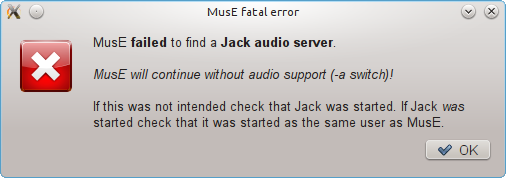
\includegraphics[width=\screenshotwidth]{pics/no_audio} 
\caption{Jack server missing}
\label{fig:no_audio} 
\end{figure}
\subsubsection{Midi only}
MusE can be started in Midi-only mode where MusE does not have any external
dependencies apart from ALSA midi. In this case start MusE from a terminal:
\shell{\$> muse2 -a}

\subsubsection{ALSA midi with Jack}
If Jack is running, by default MusE will not use ALSA devices, preferring
Jack midi instead. To force ALSA devices to be used as well as Jack
midi, start MusE with the -A option: \shell{\$> muse2 -A}

\subsection{Beginners tutorial}
To get a quick grip of what MusE can achieve please follow this beginners
tutorial.
\subsubsection{Midi Setup}
First off, fire up MusE as was described in the previous chapter, making
sure that the jack audio server is started with sufficient configuration
to allow for audio output without breakup. Also make sure your system can
make sound. 
\subsubsection{Soft synth test}
With MusE up and running right click in the Track-pane (see
Fig. \ref{fig:Main Window}) and select 
\menu{Add Synth > MESS > vam soft synth}.
A Soft Synth track called vam-0 should appear as well as a separate GUI
for the synthesizer.

Now right click once more in the Track-pane and select \menu{Add Midi
Track}. Another track appears called Track 1, and its track list Port
column should show it is bound to the synth that was just created vam-0.
If it is not, click on the Track 1 Port column to open a drop-down list
of available devices and choose vam-0.

\begin{wrapfigure}{r}{0.05\textwidth}

\includegraphics[width=0.05\textwidth]{pics/arrow_tool}
%\hrulefill
\end{wrapfigure}
Now select the drawing tool icon
from the toolbar, alternatively press the shortcut key \key{D}.
Move the mouse over to the arranger canvas as referenced in 
Fig. \ref{fig:Main Window}
and point at the midi track, the mouse should have changed to a small pencil.
Draw a Part along the midi track using the mouse. For this exercise it is
not important where or how large the drawn Part is. When you are done double
click on the drawn part. This will open up the Piano Roll editor. To the
left of the Piano Roll there are piano keys in a vertical line, try clicking
on the keys in this virtual keyboard each click should be rewarded with a
synth sound (maybe of questionable quality, a sound nevertheless) 
\begin{figure}[htp]
\centering 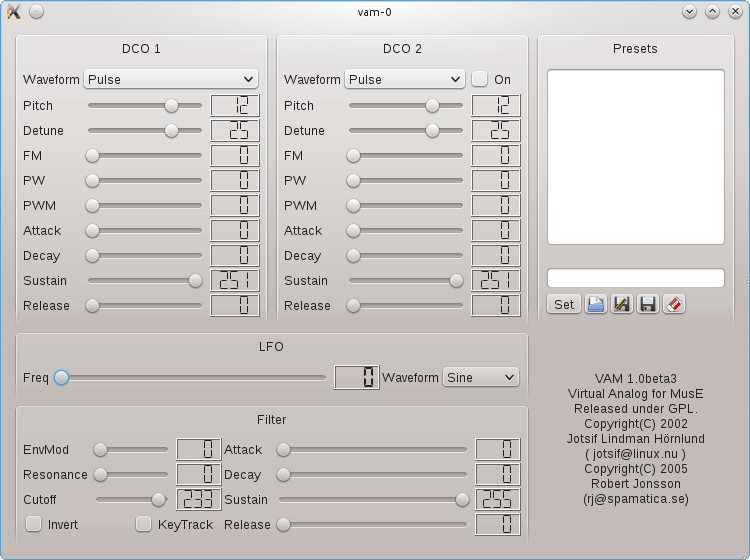
\includegraphics[width=.5\textwidth]{pics/vam_synth}
\caption{vam synthesizer}
\label{fig:vam_synth}
\end{figure}

\subsubsection{Missing sound}
If you got sound from the previous exercise you can carry on to the next,
or keep reading for further enlightenment in case you come upon trouble
later on. If there is no sound we need to do some fault hunting. First
off, click on Arranger window once more and select the vam-0 track in the
track-pane.
\begin{figure}[htp]
\centering 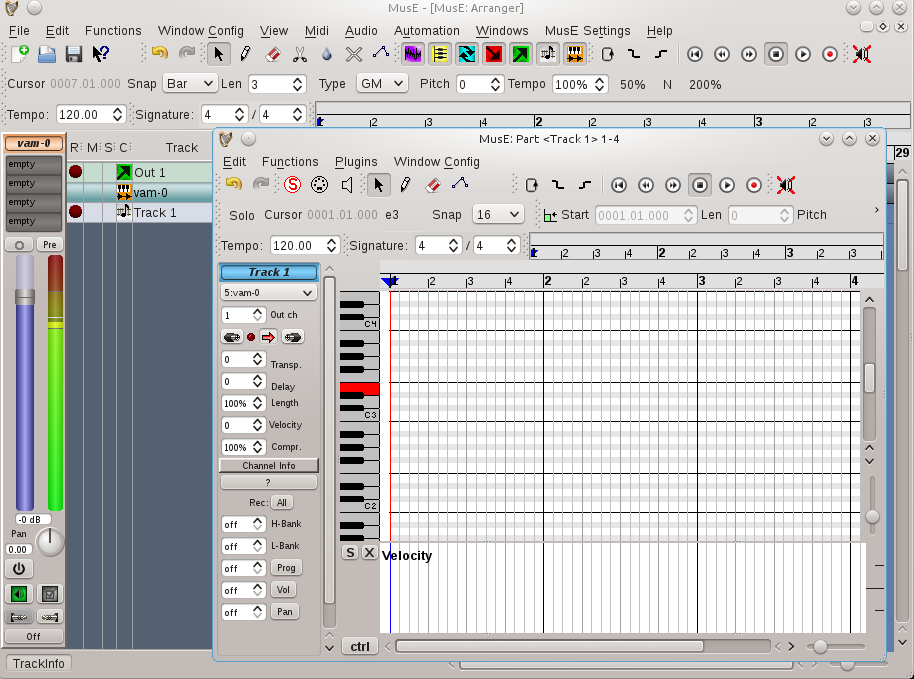
\includegraphics[width=\screenshotwidth]
{pics/main_window_with_midi_editor_vam}
\caption{Midi editor view}
\label{fig:Midi editor}
\end{figure}
Now bring back Piano Roll window and align the windows so you
can see the piano keys as well as the Meter on the Mixer Strip (see the
5 Function by function chapter for more information on these windows).
The result should be something like the following:

When pressing one of the keys on virtual Keyboard the Meter on the Mixer
Strip should light up in green to visualize that the Synth is making
sound, if it is not try to trace back your steps and and see if you did
anything differently than described.
Now, if the Meter lights up but there is still no sound we need to
check the routing between the tracks. Click on the Arranger window again
and select the Out 1 track, this is the predefined output which MusE by
default loads at startup, at the bottom of Mixer Strip there are two
buttons looking like tele- jacks, these bring up the inputs and outputs
of the track, click on the right one, the output and make sure that it is
connected to some valid outputs on your system.
\begin{wrapfigure}{r}{0.25\textwidth}
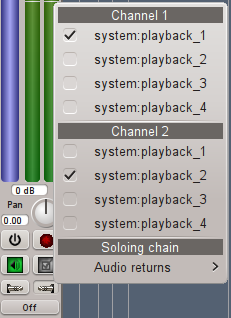
\includegraphics[width=0.25\textwidth]{pics/output_routing} 
%\hrulefill
\end{wrapfigure}
Click on the outputs to select them, if you did changes here go back and
try clicking on the Piano Roll keyboard again, hopefully it helped. If there
still are problems make sure your system actually can make sound through
Jack, this is however getting outside the scope of this manual.\\\\
\textit{This might be the time to bring up the concept of community support.
Open source software could never be what it is without the support given by
individuals on forums and mailinglists, if the information given in this
document is not enough, try googling your problem and/or get in touch with
one of the online forums for MusE or Linux audio in general. See some pointers
in the Support chapter.}


\subsubsection{Recording Midi}                                                %TODO: walkthrough of recording midi
TBD
\subsubsection{Recording Audio}
At this point we'll make a slight detour into full on audio recording. Getting
audio out of MusE has already been covered in the previous chapters so we will
concentrate on the additional steps needed to record onto an audio track.\\
\\
When MusE is first fired up, the
output track has already been created (more about this in the chapter about 
templates), to proceed with audio recording we need to add two additional tracks, a 
wave track and an input track.\\
When MusE is first started right click in an empty space on the track view
\begin{figure}[htp]
\centering 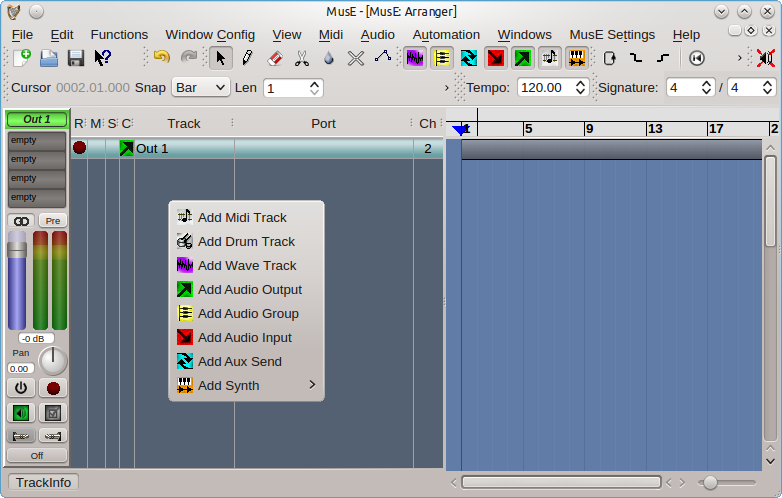
\includegraphics[width=\screenshotwidth]
{pics/main_window_add_track}
\caption{Add track}
\label{fig:Add track}
\end{figure}
and select \menu{Add Audio Input}. Right click again and also select 
\menu{Add Wave Track}. Two additional tracks are now visible in the Arranger, 
"Input 1" and "Track 1", bring up the mixer with \menu{F10} and you should see 
the following configuration.
\begin{figure}[htp]
\centering 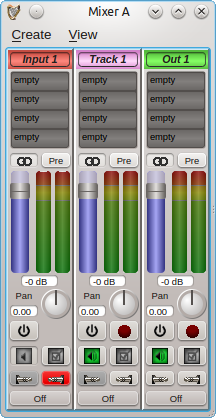
\includegraphics[width=0.25\textwidth]{pics/mixer_with_one_input} 
\caption{Mixer with one input}
\label{fig:Mixer with one input}
\end{figure}
\\
Note the buttons on each mixer strip. hover over them to see their 
functionality. For more information on all the buttons see coming chapters 
about the mixer. For now lets just do what we must.\\
1. click on the stereo symbol over the slider to change the input to a mono track.\\
2. do the same for the wave track (optional)\\
3. click on the Mute (gray speaker) icon on the input track to unmute it.\\
4. click on the input routing button (see the tooltip, it looks like a tele plug) 
on the input track and select an appropriate connection from your system.\\
5. click on the output routing button on the input track and select 
\textbf{Track 1}\\
\\
Already after the meter on the input track should be able to display that there
is incoming sound from your sound source. If there actually is sound coming 
from your sound source, that is.\\
We are now nearly ready to start recording. First we need to select a location
to store the files. MusE does not use a centralized storage of soundfiles but
uses the path of the song-file (extension .med) as guidance as to where the
audio files should be placed. Now as it happens MusE will prohibit us from
starting a recording until the songfile has been stored. So lets take advantage
of this behaviour and just go ahead and try to record. Let's get started.\\
In the mixer click on the red \textbf{record} dot on the Audio Track to arm it
for recording (or enable if you will). Now when there is audio coming into the
input it will also show up on the Audio Track. Also note that all the input and
output routing buttons on the tracks now have the same gray color, this means
that all of the tracks have a proper connection.
\begin{figure}[htp]
\centering 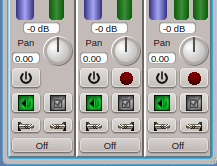
\includegraphics[width=0.25\textwidth]{pics/mixer_with_one_input_buttons} 
\caption{Mixer buttons}
\label{fig:Mixer buttons}
\end{figure}
\\
All fine and dandy. Now bring up the arranger window and find the round, red on
white  \textbf{record} button and click on it. This is your queue to MusE to
prepare for recording. However since we have not saved our song we are presented
with a dialog to do just that.\\
\begin{figure}[htp]
\centering 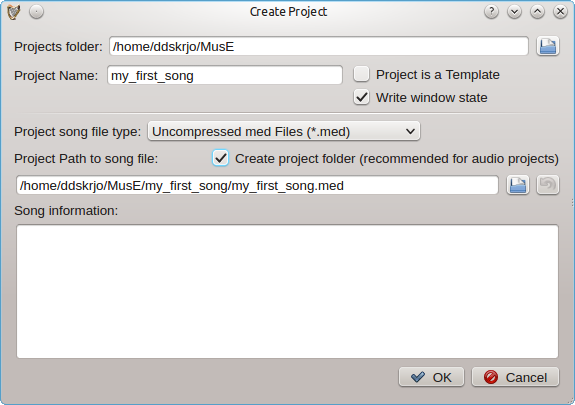
\includegraphics[width=0.6\textwidth]{pics/project_my_first_song} 
\caption{Save song}
\label{fig:Save song}
\end{figure}
Note the check box for creating a project folder, when working with audio this
is very much recommended or you may soon loose track of what audio files belong
to which song.\\
Finally we are ready to start recording! The process is completed by clicking
on the \textbf{Play} button in the Arranger. If all went well MusE then starts
to record a wave file from the Input Track placed in your song directory.\\
When you wish to stop recording press \textbf{Stop} in the Arranger, now the 
resulting waveform should be visible in the Arranger. After rewinding the Play 
position and pressing \textbf{Play} again the resulting sound should be audible
through the connected output.


\section{Basic overview}
In this section we will make a step by step walk-through of all the
different editors, their purpose and what functions they support.

\subsection{Main/Arranger}

\label{Main/Arranger} 
\begin{figure}[htp]
\centering 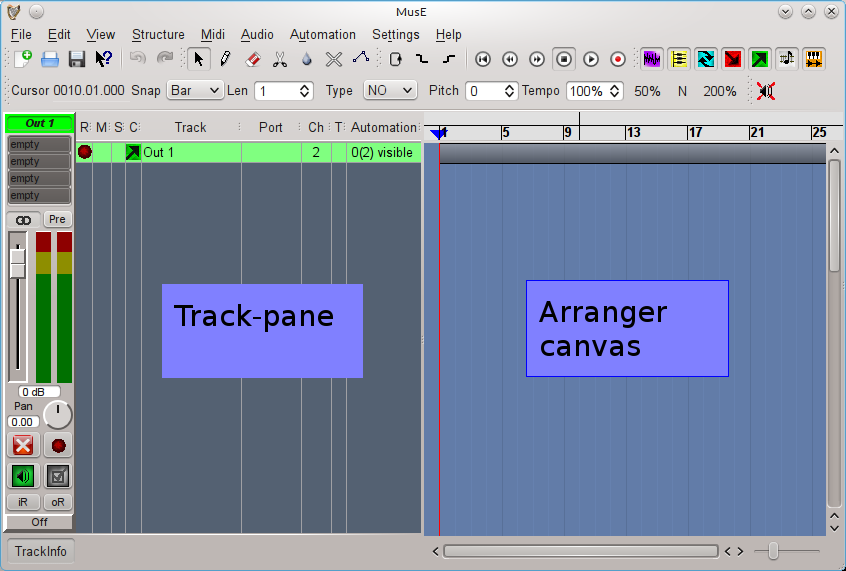
\includegraphics[width=\screenshotwidth]
{pics/main_window_annotated} 
\caption{MusE main window}
\label{fig:Main Window} 
\end{figure}
Above is the main window of MusE, the Arranger, this is what greets you
when launching MusE. The Arranger consists of two main parts, the Track-pane
and the Arranger canvas. The Track-pane lists all currently visible tracks
and the Arranger canvas contains all Parts of the composition. The
screenshot above shows an empty project. Below is MusE with a song in
progress, turns out it wasn't a very good song, but for our purposes it
is fine. In the below screenshot there are a lot of tracks visible in the
Track-pane, each have an icon which indicate it's type, wave-track, input,
output etcetera, more about that later. In the Arranger canvas a number of
parts are visible, the ones in yellow are in this composition wave files,
the multicolored line are different Parts of a drum track.

\begin{figure}[htp]
\centering 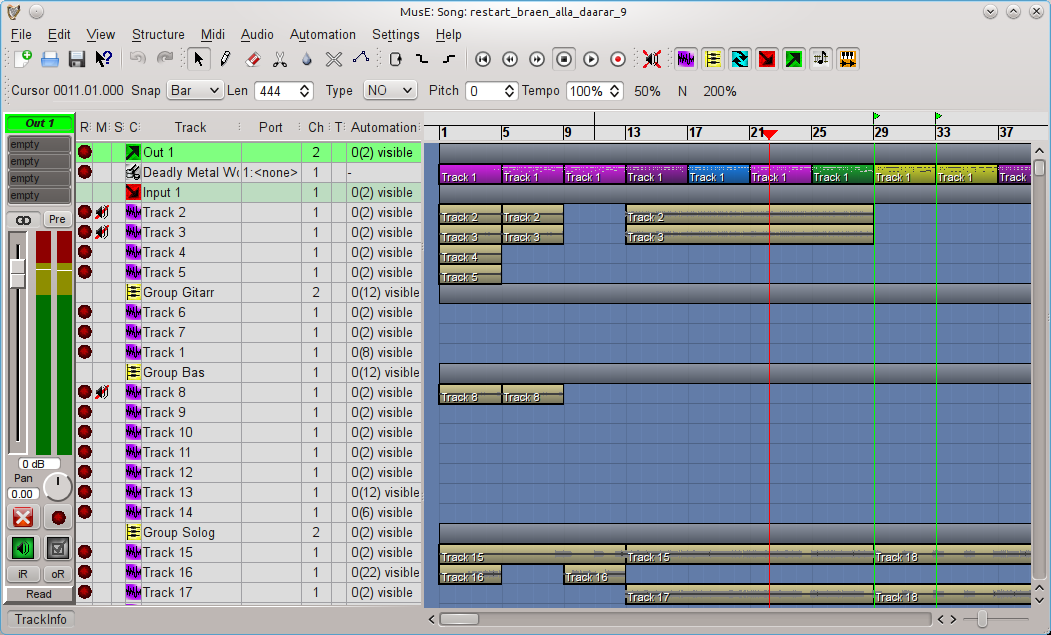
\includegraphics[width=\screenshotwidth]
{pics/main_window_with_arrangement} 
\caption{MusE main window with arrangement}
\label{fig:Main Window with arrangement} 
\end{figure}

\subsection{Mixer} \label{mixer} 
Choosing \menu{View > Mixer A} or \menu{B} from the menu in the main
window will bring up the mixer as viewed below. The mixer will open with
all options enabled, showing channel strips for all tracks in the current
setup, depending on how far you have gotten this view may become very large,
at which point it may be a good idea to limit what is viewed in the Mixer.
From the view menu all the different kinds of tracks can be toggled on/off
from the mixer. Some may find it a good idea to use the two mixers A and B
setup with different setup and store this in your song template(s), more
about this in the Song Template section. It can be argued that everything
in MusE is a track analogous to the Unix idiom that everything is a file.
The types of tracks visible in the mixer (and track-pane) are:
\begin{wrapfigure}{r}{0.5\textwidth}

\includegraphics[width=0.5\textwidth]{pics/mixer} 
%\hrulefill
\end{wrapfigure}
\begin{itemize}
\item Audio output 
\item Audio input 
\item Group track 
\item Aux track 
\item Wave track 
\item Synth track 
\item Midi track 
\end{itemize}


There is also a Midi Track variation called Drum Track, they are
however not distinguishable from Midi Tracks in the Mixer. Also the
strips for midi tracks are different in the Mixer than in the
Track-pane view.

\section{Tracks and parts}
MusE arranges your music in \emph{tracks} and \emph{parts}. The following
section shall provide you an overview of how things are done with MusE.
If you are or were a Cubase or Cakewalk user, you will feel familiar with
this. 

\subsection{Tracks}
There are two general classes of tracks: MIDI tracks and audio
tracks. MIDI tracks (and drum tracks which are internally MIDI tracks)
can hold note data. The Wave track is a type of audio track which holds
wave data. There are also several other kinds of audio tracks.

\paragraph{MIDI tracks}
MIDI and drum tracks hold MIDI event data. They don't differ much,
except that drum tracks offer a special editor which is more suitable
for drum editing.

\paragraph{Wave tracks}
They hold audio data which can be just played back or be piped through
effect plugin chains. They offer automation for these plugins.

\paragraph{Audio input tracks}
These provide the path for your audio data from outside into your
project. Set up the physical audio inputs you want to connect your
audio input track with, and then route the input tracks to various
other tracks such as wave tracks.

\paragraph{Audio output tracks}
These provide the path for your project's audio data to outside. Set
up the physical audio outputs you want to connect your audio out track
with, and then route various other tracks, such as wave tracks, to
the output tracks.

\paragraph{Audio group tracks}
Group tracks are like busses, where you can route other tracks to
them, then route the groups to other tracks. Since group tracks have
all the features of other audio tracks, like volume and pan, they
provide a convenient common routing point where you have control of
the sound before it is passed to other tracks.

\paragraph{Audio aux tracks} \label{aux_tracks} 
These provide a more convenient way to mix several audio tracks
together. With each audio aux track added, other audio tracks will
gain a common send knob for adjusting the level sent to the aux
track. This can be more convenient than using several group tracks.

\paragraph{Synthesizer tracks}
This type of track is a software synthesizer which MIDI and drum tracks
can be assigned to.

\paragraph{Creation}
You can create a track by either right-clicking in the arranger's track   % TODO: insert screenshot
list and then adding the desired track, or via the edit menu.

\paragraph{Attributes}                                                    
Tracks have several attributes:
\begin{description}
\item [{Mute:}] If you click on the \emph{Mute} field (denoted with
a "M" column header), the track gets muted and stops producing sound.
\item [{Solo:}] \label{track_attr_solo} The solo button ("S" column
header) singles out a track for listening. It mutes
some other tracks but may phantom solo others. 
For more info see the section on soloing: \ref{track_soloing} and
phantom soloing: \ref{phantom_soloing}
\item [{Record:}] The R column "arms" your track for recording.
When you rec-arm your song and have no tracks rec-armed, you won't be
able to record anything. See also the config option "move rec-arm with    % TODO: reference to rec-arm config option
selection". 
\item [{Track name:}] Double-click to edit the track name.
\item [{Port:}] For MIDI tracks, this lets you select the MIDI
port to which the events should be routed. This can be your physical
synthesizer or a software synthesizer. For soft synths, this is the
port the synth is associated to. For other track types, this is disabled.
\item [{Channel:}] For MIDI tracks, this is the MIDI channel the
output is sent to. For any kind of audio tracks, this is the number of
channels (mono, stereo).
                                                                          % TODO: what's that "T" column?!
\item [{Automation:}] \label{track_attr_automation} For audio tracks,
this lets you set up the automation display in the arranger. 
(See automation \ref{audio_automation}). Clicking this will provide you
with a popup menu with lots of submenus. Clicking on a submenu will
select or unselect it showing or hiding the automation parameter as a 
graph overlaid on top of the track.\\
The submenus let you select the color you want to associate with the
automation parameter. There you can also assign midi controllers to
the parameters, a dialog is shown where you can manually choose the
midi controller, with a \emph{learn} button to 'listen for' and
automatically recognize any midi controller operated by you.

\item [{Clef:}] For MIDI tracks, you can specify a clef here. This
only affects the score editor.

\end{description}

\subsubsection{The trackinfo side bar}
In the arranger and the part editors, you'll have a trackinfo sidebar
on the left side. You can set up track-type specific things there.

\paragraph{MIDI trackinfo sidebar} \label{midi_trackinfo_sidebar}
The MIDI trackinfo sidebar lets you change program, volume, pan and
more. This sidebar can also be viewed at the left of the pianoroll
editor.                                                                        %%FIXME Ref to pianoroll
\subparagraph{Old style drum tracks:}
These are MIDI tracks as well, but with a few differences. They allow
you to map certain drum sounds with different input notes, and you
can change the output settings of a certain "drum instrument" without
having to alter each single event.

However, they have certain limitations: They only can handle 128 sounds
(even if you have more synthes), they aren't really compatible with
MIDI tracks (you can interchange parts between them, but if you touched
the drum list, you'll get unexpected results), you can't set a program
for the used channel and more.

\subsubsection{New style drum tracks}
Because of these limitations, we introduced the new-style drum tracks.
They're not fully compatible with the old drum tracks, so the old are
still retained. Under "Global Settings", "GUI settings", you can set
up whether you prefer the old or new.

They are handled exactly like plain MIDI tracks (staying compatible with
them), and offer all of the functionality, though in a different way.
They allow you to re-order the drum map efficiently, you can open parts
from multiple drum tracks in \emph{one} drum editor (MusE will separate
the sounds from different tracks according to your settings, see the
"Window Config" menu), and you can set programs as with normal MIDI tracks.

\subparagraph{MIDI trackinfo controls:}
\begin{description}
\item [{Output port:}] This drop-down list selects the midi port
to send midi output from this track. 
\item [{Output channel:}] This box selects the midi channel to be
used on the output port.
\item [{Input and output routing:}] Selects midi ports and
channels to receive midi from, and soloing paths. (See Routes
\ref{routes}).
\item [{Midi through:}] This button selects whether midi input is
passed through to the selected output port.\\
Depending on your midi devices and settings, there are cases when
this should be off such as using the same port and channel for
input and output (otherwise a double-note \emph{echo} will be heard),
and cases when it must be on such as when using a synthesizer track
as output device. 
\item [{Input detect indicator:}] Blinks when midi activity is
detected on the selected midi channels on the selected midi input
ports.
\item [{Transpose:}] This transposes midi input notes up or down
in pitch. This is very useful if your midi keyboard hasn't enough
keys or the selected output device plays an octave too low or high,
and you would like to shift the octave of the incoming notes to
compensate.
\item [{Delay:}] Adjusts the delay of the notes.                               %% FIXME What is this again? Does it work?
\item [{Length:}] Adjusts the length of the notes.                             %% FIXME What is this again? Does it work?
\item [{Velocity:}] Adjusts the velocity of incoming notes.
Use it to compensate for a too-loud or too-soft keyboard.
\item [{Compression:}] Adjusts the compression of incoming note
velocities. Use it to make soft incoming notes louder, and loud
notes not so loud. 
\item [{Instrument:}] Selects the midi instrument patch to be used
by the selected output port. This is equivalent of dialing the patch
in the bank and program boxes, except it displays a more friendly
patch \emph{name} as defined by the selected output port's midi
instrument. See instruments, or port configuration                             %% FIXME Ref to instruments. 
\ref{midi_port_config}
\item [{H-Bank:}] Selects the high bank number of the current patch.
\item [{L-Bank:}] Selects the low bank number of the current patch.
\item [{Prog:}] Selects the program number of the current patch.
\item [{Volume:}] Adjusts the midi volume controller.
\item [{Pan:}] Adjusts the midi pan controller.
\end{description}
The buttons beside the Prog, Volume, and Pan boxes store the value,
at the current transport position, for midi automation. (See
automation \ref{midi_automation}).

Note that the 'Prog' button stores H-Bank and L-Bank along with
'Prog' value, so there are no H-Bank and L-Bank buttons.

The 'All' button simply stores all three Program (and banks), Volume,
and Pan values at once.

\emph{Tip:} If the Song Type is GM, GS, or XG, you may need to store           %% FIXME Ref to song type
desired values at transport position zero, otherwise your adjustments
may be overridden by the instrument when the transport is moved back
to position zero. If this behaviour is undesired, you can set the 
Song Type to 'NO' meaning no song type.                                        %% FIXME Ref to explanation of instruments and default controller values

\paragraph{Audio trackinfo sidebar}
Unlike the midi trackinfo sidebar, the audio trackinfo side bar
is nothing more than an embedded audio mixer strip, the exact same 
strip as found in the mixers. (See mixer \ref{mixer}).
\subparagraph{Effects rack:}
On the top of the audio trackinfo sidebar, there is an effects rack
which allows you to apply various plugins on the audio. For more
information on this, refer to \ref{effects_rack}.


\subsection{Parts}
Within MIDI, drum and wave tracks, you can create \emph{parts}. Parts
are chunks of coherent notes or wave data which can be moved around,
copied, cloned and deleted independent from other parts.

Parts are created by selecting the pencil tool and then drawing onto
the right part area in the arranger. You can move them with the arrow
tool, delete them using the \key{DEL} key, and a right-click opens
a popup menu. This menu allows you even more stuff, such as setting
the part's color, saving the part to disk etc.. You can use
\key{CTRL+C} and \key{CTRL+V} for copying and pasting parts.
\key{CTRL+B} pastes the part as a clone. Pressing \key{SHIFT}
additionally provides you a dialog which allows you to paste the part
multiple times and set more stuff.

You can also copy parts with the mouse by moving the part with the mouse
while holding down the \key{CTRL} key.


\section{Routes} \label{routes}
Routes are how tracks are connected together and to the outside world.
(They are also how Jack midi ports connect to the outside world. See
midi port configuration \ref{midi_port_config}).
Each track strip has two buttons whose icons look like plugs. One button
is for input routing and the other is for output routing. Clicking on
these buttons will pop up a menu of available input or output routes that
you can connect to. Most audio tracks list other tracks to connect to, 
but audio input and output tracks are special: Audio input track input
routing menus list available Jack audio input ports. Conversely audio
output track output routing menus list available Jack audio output ports.

\begin{wrapfigure}{r}{0.25\textwidth}
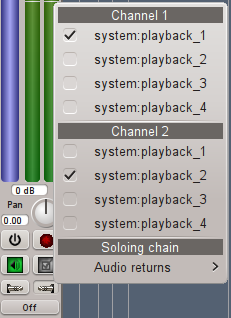
\includegraphics[width=0.25\textwidth]{pics/output_routing} 
%\hrulefill
\end{wrapfigure}

Meanwhile MIDI and drum tracks allow you to route available MIDI ports
and channels to the track using a handy popup matrix.

\begin{wrapfigure}{r}{0.25\textwidth}
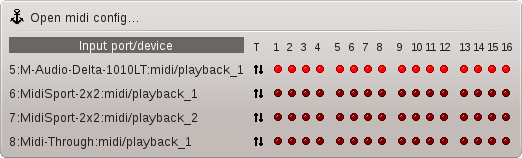
\includegraphics[width=0.25\textwidth]{pics/midi_routing_matrix} 
%\hrulefill
\end{wrapfigure}


\subsection{Anti circular routing} \label{anti_circular_routing}
Any routing menu item which would cause a circular routing condition
is grayed out. Find out why the condition would exist by examining 
routing paths involved and correct the situation if required.

Also, you cannot use a track's aux sends if the track has an input
route path from ANY Aux Track. (See aux tracks \ref{aux_tracks}).
Aux send knobs and labels are disabled in that case.

\subsection{Soloing chain routes} \label{soloing_chain_routes}
Soloing chains (see solo chains \ref{soloing_chains}) are really just
routes like any other. The available solo chaining paths are displayed
in the routing popup menus.

\section{Track soloing} \label{track_soloing}
Soloing allows you to single out a track for listening while muting others,
without you having to mute the other tracks. (See soloing track attribute
\ref{track_attr_solo}).

\subsection{Phantom soloing} \label{phantom_soloing}
In order to solo a track and mute others so that it is heard, MusE
employs 'phantom' soloing: When a track is soloed, MusE automatically
solos all tracks routed to and from this track. (See routes
\ref{routes}). A phantom soloed track is indicated by a black square
in the track pane solo column. (See track attributes
\ref{track_attr_solo}).


\begin{figure}[htp]
\centering 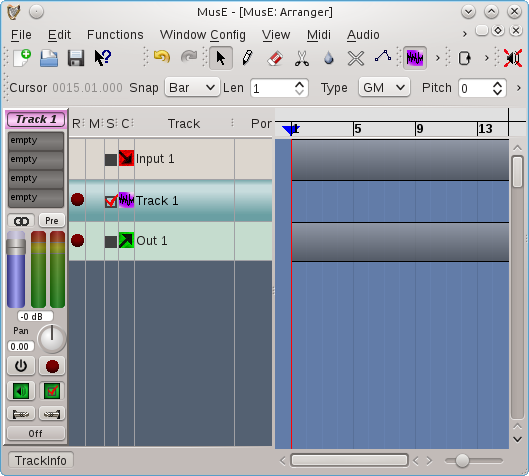
\includegraphics[width=\screenshotwidth]{pics/soloing_window}
\caption{Soloing, with phantom soloing}
\label{fig:Soloing} 
\end{figure}

\subsection{Soloing chains} \label{soloing_chains}
When an audio output track sends audio to some external entity, such
as an external running application, and audio from the external entity
is fed back into a MusE audio input track, solo chains allow you to
solo the input or output, and MusE will complete the path automatically
soloing the other, and all paths that came before or after it.

Solo chains also work with MIDI tracks chained to audio inputs:
When a MIDI track drives some MIDI device whose audio is fed into MusE,
solo chains allow the entire chain to be soloed.

Solo chains are accessed via routing menus. (See solo chain routes
\ref{soloing_chain_routes}).

\section{Plugins} \label{plugins}
Plugins are small add-ons which can process a track's data.

MIDI plugins operate on midi and drum tracks, and are found in
the \menu{Midi} menu.

Audio plugins can be applied to any track handling audio (that is,
inputs, outputs, wave tracks, synth tracks). The effects rack
section describes this. (See effects rack \ref{effects_rack}).

\subsection{The audio effects rack} \label{effects_rack}
All audio track types (Input, Output, Group, Wave, Synth, and Aux) have
an effects rack into which audio plugins can be inserted in a chain.
Currently each rack can accommodate up to four plugins.

MusE currently supports LADSPA plugins and DSSI synth and effects
plugins.

Plugins can be added by double-clicking on an entry in the effect rack
in the track info pane (which is shown at the left side of the arranger
when the according track is selected). Right-clicking the rack items
offers a self-explanatory popup menu.

All plugin controls can be automated. (See audio automation
\ref{audio_automation}).

One must carefully consider how many audio inputs and outputs a plugin
has, and how may channels the particular audio track has (1 mono or
2 stereo), and how MusE uses the plugins in the rack.

Learn more about this in the appendix Understanding the Effects Rack:
\ref{apx_effects_rack}

\subsubsection{Audio plugin Graphical User Interfaces (GUIs)} 
\label{plugin_guis} Once a plugin is added, you need a way to 
manipulate its controls, which affect its behaviour and operate
on the sound.

MusE can show a generic GUI which contains all of the
plugin's controls arranged in a rather plain generic fashion.

Some plugins may also have a native GUI which looks much better (it
was specifically designed for the plugin).

Both GUI types are opened from the effects rack right-click popup menu.

\section{Automation} \label{automation}
Automation is the ability to record (or construct) and playback
exact sequences of control movements.

MIDI and audio automation are each currently uniquely different,
but share some similarities.

\subsection{Audio automation} \label{audio_automation}
Almost all graphical audio controls in MusE can be automated.

This includes an audio track's volume and pan, and the controls
of any plugins in the effects rack, and if the track is a
synthesizer track, all of the synth's controls.

Each control has a manual adjustment value. This value is shown
when there is no automation data at all, or automation has been
disabled.

For plugin and synth controls, it is usually more desirable to
manipulate automation with the generic plugin GUIs, because
MusE has full control over their behaviour. (See plugin GUIs
\ref{plugin_guis}).

There are a few ways to enter audio automation data:
\begin{itemize}
\item By adjusting audio controls while the transport is rolling.
MusE will record the exact movements.
\item By adjusting audio controls while the transport is stopped,
at different transport positions. TOUCH mode allows this.
\item By right-clicking any audio control and choosing an operation
from the automation popup menu. This includes storing, erasing,
and clearing automation events, and seeking the next or previous
event.
\item By drawing the data on the audio track's automation graphs.
(See track automation \ref{track_attr_automation}).
\end{itemize}
\paragraph{Audio automation modes} 
Each audio track strip has an automation mode button
at the bottom. There are four automation modes:
\begin{description}
\item [{OFF:}] Disables all automation, uses manual value always.
\item [{READ:}] Automation data is applied to controls. If any
automation data exists, the manual value is overridden and has
no effect.
\item [{TOUCH:}] Allows you to alter a control at any time, while
transport is stopped or rolling, If rolling, when the control is
released it returns to reading from automation data. 
\item [{WRITE:}] Allows to adjust an initial value before rolling
the transport. While rolling, when the control is released it does
not return to reading from automation data. 
\end{description}
Here is a screenshot of automation WRITE mode, and some automation
data, with the track pane automation popup menu showing (see track
automation \ref{track_attr_automation}):
\begin{figure}[htp]
\centering 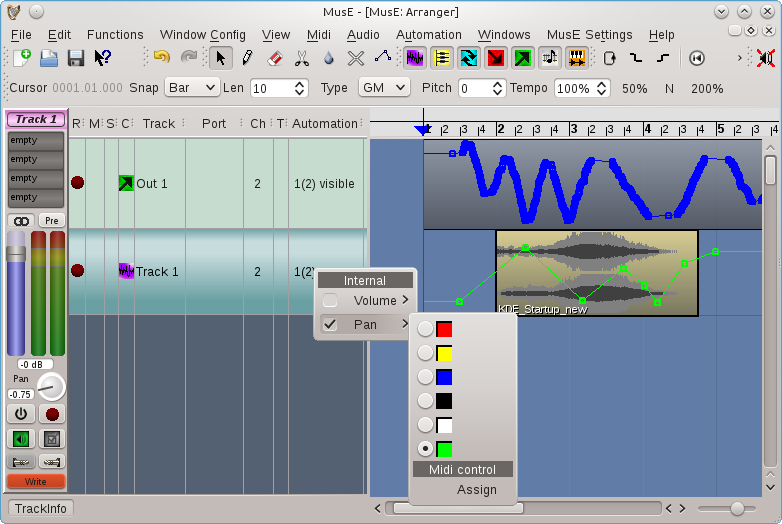
\includegraphics[width=\screenshotwidth]
{pics/main_window_with_automation}
\caption{Audio automation graphs}
\label{fig:audio_automation} 
\end{figure}

\label{midi_automation} \subsection{Midi automation} 
MIDI automation is a slightly different concept: Unlike audio
automation, currently there is no automation 'mode' and it doesn't
record graphical control movements. Data is viewed from within
the pianoroll and drum editors, by clicking on the 'Ctrl' button               %% FIXME Ref to pianoroll
on those canvases.
                                       
Similar to audio controls, each midi control has a manual adjustment
value. This value is overridden when there is midi automation data.

There are a few ways to enter MIDI automation data:
\begin{itemize}
\item By adjusting external MIDI controls (such as a midi keyboard
pitch or modulation wheel) while the transport is rolling and both
the transport and midi track are in record mode. MusE will record
the exact movements. As mentioned earlier, note that graphical control
movements are not recorded.                                                    %% FIXME Feature requests for true midi automation
\item By right-clicking any midi control and choosing an operation
from the automation popup menu. This includes storing and erasing
automation events.                                                             %% FIXME Store/erase not enough functionality
\item By adjusting volume, pan, bank or program boxes in the midi
trackinfo panel and clicking the corresponding volume, pan, or 
program buttons. (See midi trackinfo \ref{midi_trackinfo_sidebar}).
\item By drawing the data on a midi part's automation graphs.
\end{itemize}
Here is a screen shot of a midi track, containing a midi part
which has been opened with the pianoroll editor and automation                 %% FIXME Ref to pianoroll
data showing.
                                                         
The 'Ctrl' popup menu (bottom left) shows available midi controllers
and the green dot indicates there is some data.

\begin{figure}[htp]
\centering 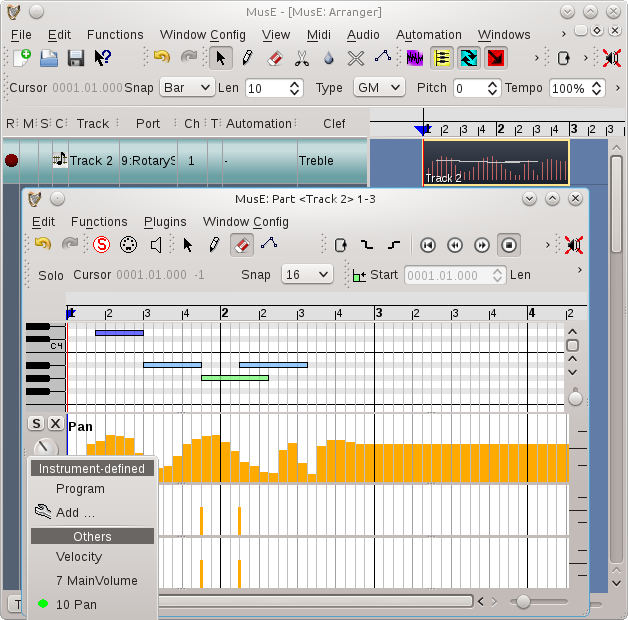
\includegraphics[width=\screenshotwidth]
{pics/main_window_with_midi_automation}
\caption{MIDI automation graphs}
\label{fig:midi_automation} 
\end{figure}
 

\section{Configuration}

\subsection{MIDI ports} 
MIDI ports provide an abstraction layer for your MIDI hardware and
synthesizers (which can be both software and hardware synthesizers),
and other MIDI applications. Port are numbered. In order to produce
sound, each MIDI track is assigned to exactly one MIDI port, to which
the MIDI events are then sent.

The advantage of this abstraction layer is that if your system changes,
for example you change MIDI hardware, then you need only modify the
ports instead of all the tracks using those ports. This is similar
to the audio input and output track abstraction to the outside world.

\label{midi_port_config} \paragraph{MIDI port configuration} 
In the midi/softsynth configuration menu, you must map the port numbers
to the actual devices (by selecting ALSA or jack midi ports, or synth
plugins).

Try left-clicking on the "Ports" column of some MIDI track.
If you use a soft synth, right-clicking the Ports column of the synth
or any track using the synth lets you launch the synth's GUI.

\begin{figure}[htp]
\centering 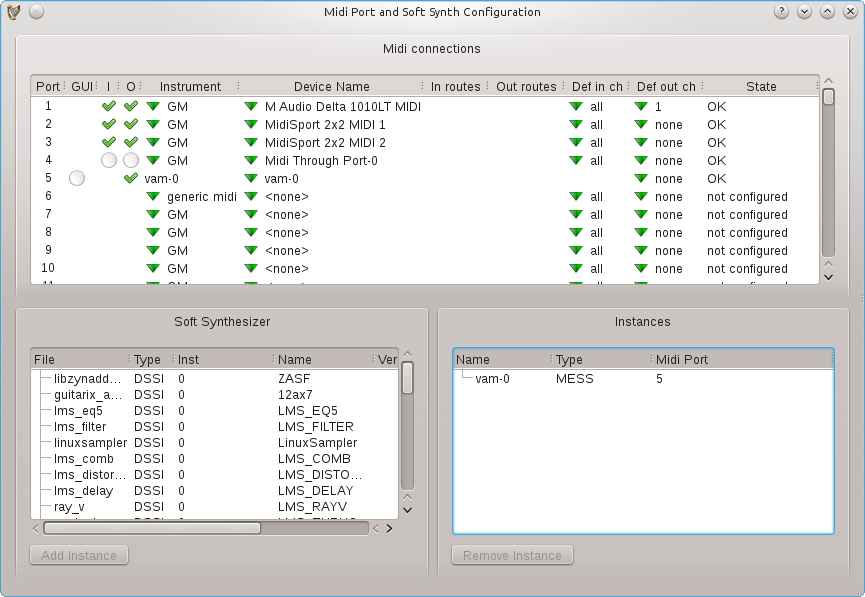
\includegraphics[width=\screenshotwidth]
{pics/midi_config_window} 
\caption{Midi configuration window}
\label{fig:midi_config_window} 
\end{figure}

\paragraph{Columns in the MIDI configuration ports list:}
\begin{description}
\item [{GUI:}] For synthesizer devices, indicates if a gui is available
and if it is showing. Click to show.
\item [{I:}] If present, the port can accept MIDI input. Click to
enable or disable it.
\item [{O:}] If present, the port can send MIDI output. Click to enable
or disable it.
\item [{Instrument:}] Selects the instrument to be used when MIDI is
played through the port.
\item [{Device name:}] Selects or creates a MIDI device assigned to the
port. These can be Jack MIDI devices or ALSA MIDI devices (if ALSA is
enabled), or soft synthesizers. Jack MIDI devices are created by selecting
Create Jack Device from the Device name drop-down menu. Jack MIDI devices
can be renamed as you wish by clicking the device name. Soft synthesizers
are created by clicking in the soft synthesizer list and then Add
Instance. Or you can simply create a new synthesizer track from the
arranger track list, or even the mixer menus.
\item [{In and Out routes:}] These are for Jack MIDI devices, they are
the routes to and from available Jack MIDI ports. Jack may provide
different alias names for these ports, you can select which alias
is shown.
\item [{Default in channels:}] Auto-connect these port channels to
new midi or drum tracks.
\item [{Default out channel:}] Auto-connect new midi or drum tracks
to this channel on the port.
\item [{State:}] Indicates the state of the port including any errors
opening it.
\end{description}

\subsection{Global settings}
\subsubsection{Audio settings}
\paragraph{Minimum control period}
Plugins can usually process an arbitrarily small (or large) amount
of samples. If some plugin control value changes continuously, to provide
ideal listening experience, MusE would need to call the plugin 44100
times a second, asking for one single value at a time. With the minimum
control period setting, the user can force MusE to ask the plugin for
at least N values. Setting this value to 64 would in this situation
make MusE call the plugin $689=\frac{44100}{64})$ times a second,
asking for 64 values at a time. While doing this will reduce accuracy
of control changes, it may also reduce CPU usage, because calling
the plugin more often, requesting smaller chunks, is more expensive
than calling it seldomly, requesting larger chunks.
\subparagraph{Recommendation}
If you have no performance problems, or if you want to do the final
downmix of your project, set this to a low value. If you're experiencing
performance problems, increasing this value might help.

\chapter{Appendix}
\label{apx_effects_rack} \section{Understanding the effects rack} 
One must carefully consider how many audio inputs and outputs a plugin
has, and how may channels the particular audio track has (1 mono or
2 stereo), and how MusE uses the plugins in the rack.

MusE will try to internally create as many independent copies
(instances) of a plugin as necessary, to satisfy the number of channels
in the audio track.
Basically it divides the number of track channels by the number of 
plugin audio inputs or outputs to determine how many copies to make.
First it examines the number of plugin audio outputs, and if there are
none, it will examine the number of audio inputs, and if there are
none, it will simply use just one plugin copy.

For mono tracks with plugins having more than one audio input or
output, MusE uses the first input or output and ignores the rest. 

For stereo tracks:

\begin{tabular}{|c|c|c|c|c|}
\hline
plugin inputs & outputs & copies & track in route channels &
track out route channels\\
\hline
\hline
0 & 0 & 1 & 0 & 0\\
\hline
0 & 1 & 2 & 0 & 2\\
\hline
0 & >=2 & 1 & 0 & 2\\
\hline
1 & 0 & 2 & 2 & 0\\
\hline
1 & 1 & 2 & 2 & 2\\
\hline
1 & >=2 & 1 & 1 (L only) & 2\\
\hline
>=2 & 0 & 1 & 2 & 0\\
\hline
>=2 & 1 & 2 & 2 & 2\\
\hline
>=2 & >=2 & 1 & 2 & 2\\
\hline
\end{tabular}

Notice that on a stereo track with a plugin having one audio input and
two audio outputs, only the first track input route channel is used
(left only).
 
These same rules apply to inter-plugin audio when more than one plugin 
is in the rack chain. Extra audio outputs of one plugin may be ignored
by the next plugin if not used. 
 
Currently specialized plugins with many inputs and/or outputs are not 
really useful in MusE.

Nor are so-called 'realtime' control plugins which use audio inputs 
and outputs for control signals. 

Loud noise alert! Beware of using such plugins in an audio effects
rack. 

Example: Consider a stereo Audio Input track with these effect rack 
 LADSPA plugins: 
 
\begin{itemize}
\item comb\_splitter Comb Splitter by Steve Harris
\item tap\_stereo\_echo Tap Stereo Echo by Tom Szilagyi
\end{itemize}
    

The Comb Splitter has one audio input and two audio outputs. 
The Stereo Echo has two audio inputs and two audio outputs.
  
The stereo Audio Input track will therefore ignore its second
input route connection. It will process the left input only,
separating it into stereo with the Comb Splitter, passing the  
split stereo signal into the Stereo Echo, finally producing 
stereo output available at the Audio Input track's output routes.      
  
  
One improvement would be not creating unused redundant plugin copies
between plugins in stereo tracks.
For example, for a plugin having one audio input and one audio output,
feeding a plugin having one audio input and two audio outputs,  
the extra copy of the first plugin is redundant and not required,
but currently it is created anyway.
\end{document}

